\documentclass[letterpaper,12pt]{article}
\usepackage{tabularx} % extra features for tabular environment
\usepackage{subfig}
\usepackage{makecell}
\usepackage{listings}
\usepackage{color}
\usepackage[utf8]{inputenc}
\usepackage[T1]{fontenc}
\usepackage{textcomp}
\usepackage{float}
\usepackage{xcolor}
\usepackage[top=0.8in,bottom=0.8in,left=1.2in,right=0.6in]{geometry}
\usepackage{amsmath}  % improve math presentation
\usepackage{graphicx} % takes care of graphic including machinery
\usepackage[margin=1in,letterpaper]{geometry} % decreases margins
\usepackage{cite} % takes care of citations
\usepackage[final]{hyperref} % adds hyper links inside the generated pdf file
\hypersetup{
	colorlinks=true,       % false: boxed links; true: colored links
	linkcolor=blue,        % color of internal links
	citecolor=blue,        % color of links to bibliography
	filecolor=magenta,     % color of file links
	urlcolor=blue         
}
\usepackage{blindtext}
%++++++++++++++++++++++++++++++++++++++++


\begin{document}

\title{Predicting the Popularity of Online News}
\author{Anyu Zhu, Zhuofan Li, Yuanyuan Zheng, and Xiao Tan\footnote{Every group member equally contributed to the completion of this project.}}
\date{\today}
\maketitle

\begin{abstract}
Nowadays, more and more people enjoys reading and sharing online news articles. The number of shares under a news article is one of the critical indicators of how popular the news is. In this project, we intended to find a prediction model for online news popularity and set of related features, using regression techniques. We explored the data set 'Online News Popularity' retrieved from UCI Machine Learning Repository. We applied Linear Regression, Generalized Linear Regression, and Kernel Method. Their performances are recorded and compared. Our work can help media companies to predict news popularity before publication.

\textbf{Keywords: } Regression Analysis; Feature Selection; Model Selection

\end{abstract}

\newpage
\tableofcontents

\newpage
\section{Introduction}
In 21st century, reading and sharing news is now becoming the center of people’s entertainment lives. Thus, it is of increasingly importance for reporters to predict the popularity of the articles before publishing. For the purpose of this paper, we intend to make use of a largely collected data set with over 39000 articles from UCI Machine Learning Repository. We first selected informative features based on regression models, then analyzed and compared the performance of these prediction methods.

This paper started with most basic linear regression methods, incorporated a broader and more abstract set of features, and gradually transformed to more generalized classification methods: logistic regression. Finally, we applied kernel methods to the data based on feature selection results of fisher score. In evaluation part, by dividing data into training and testing set, we compared the prediction accuracy of the three models. In the last section, we discussed possible future work.

\section{Data Preparation}
\subsection{Dataset Description}
The dataset contains a set of features related to articles posted by online news website Mashable over a span of 2 years, acquired on January 8, 2015. It contains over 35000+ records with 61 attributes. The attributes can be basically divided into four categories \cite{a1}:
\begin{itemize}
    \item Basic information: such as URL of the post, number of tokens in title, content, average length of the words used etc.
    \item Detailed information about the content: such as number of images, videos, referencing links with the same web page and other web pages, number of keywords etc.
    \item  News category information: such as the category (business, lifestyle, entertainment, tech, social media, world) and the time in which day of week the article was posted 
    \item Analysis information from NLP: such as LDA, subjectivity, positivity, negativity, polarity and best, worst and average keyword
\end{itemize}
We define the last attribute: shares, as our parameter representing the popularity of online news, thus our target data. This dataset does not share the original content but some statistics associated with it. The original content be publicly accessed and retrieved using the provided urls (first attribute).

\subsection{Data Preprocessing}
In this section, we applied several techniques to deal with the inconsistent data, missing data, and inappropriate data. 

First, we noticed that there are a few records with attribute n\_tokens\_content equal to 0, which means the number of words in the articles' content is zero. Thus, they were regarded as invalid records and deleted from the dataset and considered as missing data. The attribute n\_non\_stop word means rate of non-stop words in the content, which should be between 0 and 1, there is one record with value 1042, and was considered as inappropriate data which should be removed. We then analyzed the skewness of target variable (34.95), and should be considered as severely skewed. Thus log transformation is applied as fig.\ref{fig1}:
\begin{figure}
\centering
    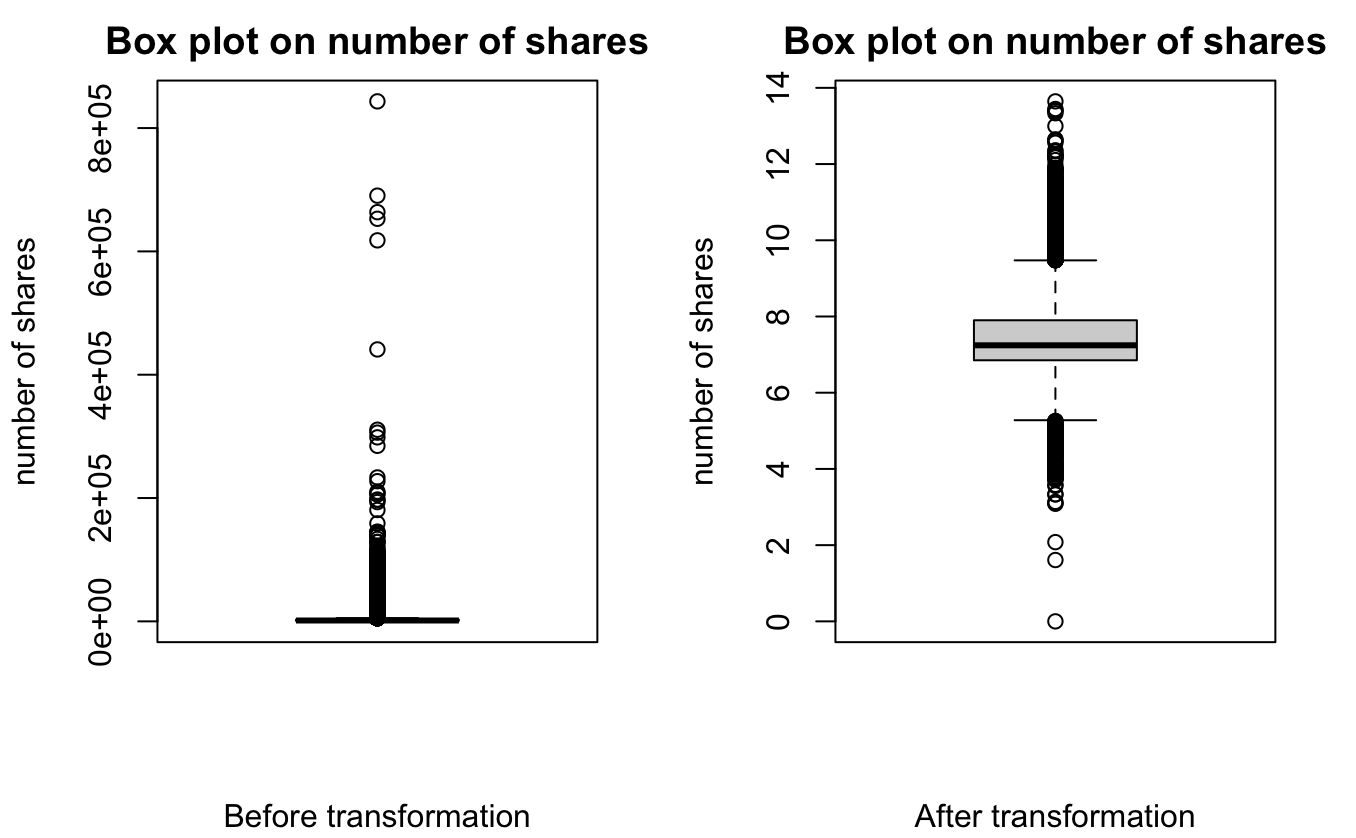
\includegraphics[width=0.7\linewidth]{1.png}
    \caption{Log Transformation}
    \label{fig1}
\end{figure}

From the figure \ref{fig1} we can see after transformation for the target variable, the skewness is significantly reduced and there are still many variables which will be hard for a linear regression to predict the exact number of shares. Further process of handling of the target variable for model building is discussed in the modeling section. 

Then we moved on to remove the outliers in target variable. Based on results of the box plot statistics, the lower outer fence and the upper outer fence is constructed using the fence measure to consider the mild outliers and exclude the extreme outliers. After this step, the box plots are as fig.\ref{fig2}:
\begin{figure}
\centering
    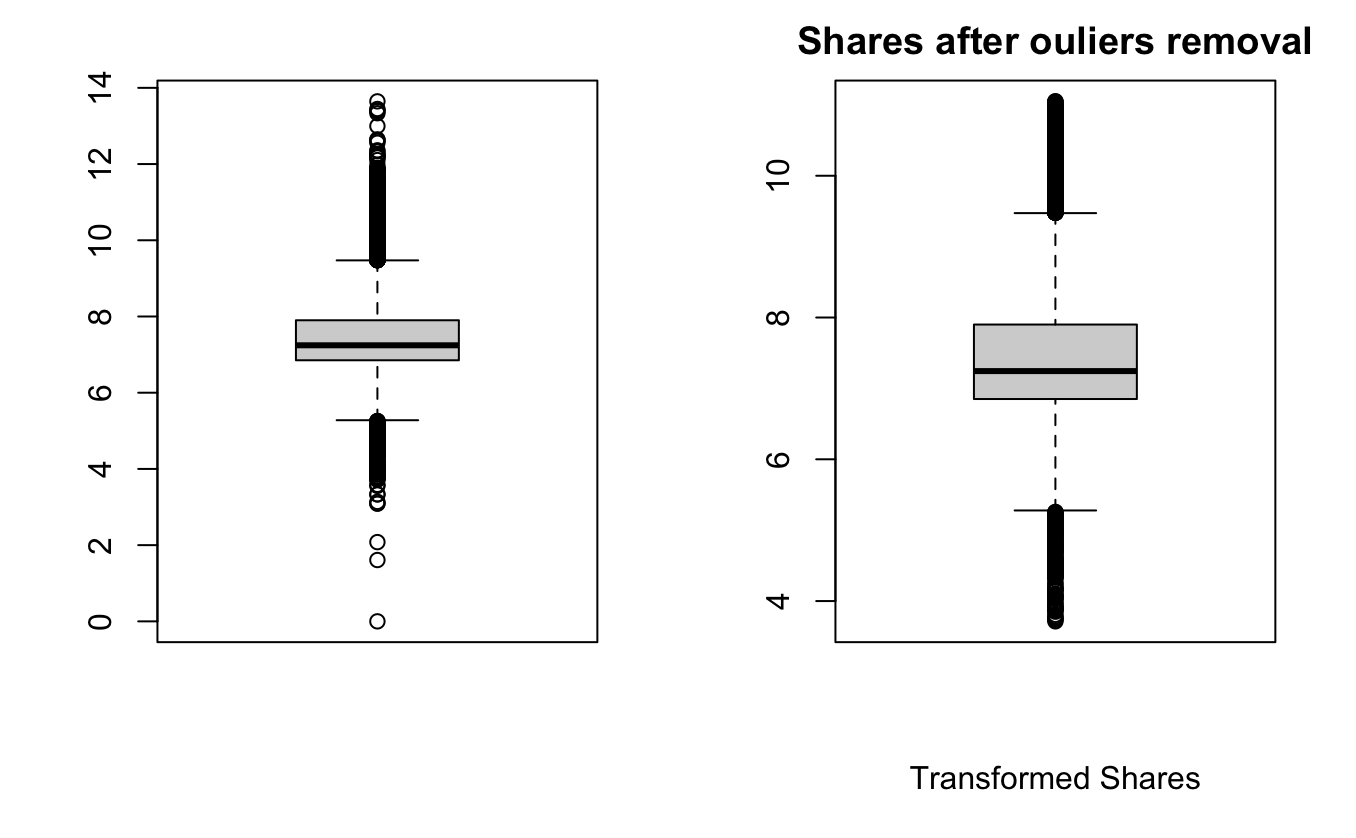
\includegraphics[width=0.7\linewidth]{2.png}
    \caption{Outliers Removal}
    \label{fig2}
\end{figure}
This step removed records with too many or too few number of shares, and the data is ready for regression analysis. In the final results' comparison section, we divided the data set by 80\% and 20\%, as training and testing set separately.

\section{Methods}

\subsection{Linear Regression}
In this section, we applied basic linear regression to the modified data set.
\subsubsection{Feature Selection}
All the attributes in the data set are numeric (some are one hot encoded), so linear regression model is built to predict an exact value of the target variable. Applying all the predictors to the model results in some NA value coefficients, which indicates that there are multi-colinearity between some predictors, such as “Weekend” and other weekdays. After deleting these predictors, the variables are selected based on variance inflation factors. After the selection, 38 predictors are preserved.

Function “regsubset” from package “leaps” is used to select the appropriate model. The selection criterion is set as BIC, because it tends to select the model with less predictors when the total number of instances is large, and since there are many predictors, a simpler model that is easy to comprehend is preferred. In the end, the model with 26 predictors prevails as shown in fig.\ref{fig6}.
\begin{figure}%
    \centering
    \subfloat[Before selection]{{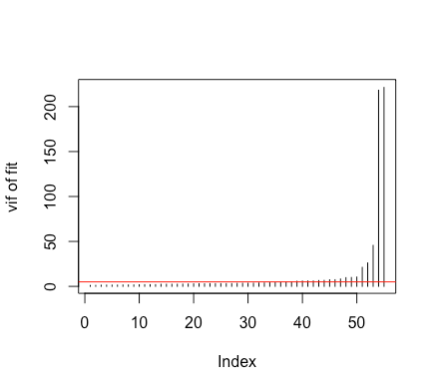
\includegraphics[width=5cm]{6.1.png} }}%
    \qquad
    \subfloat[After selection]{{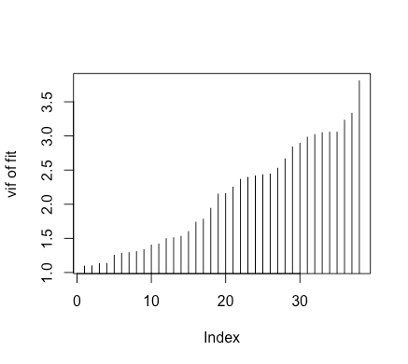
\includegraphics[width=5cm]{6.2.png} }}%
    \caption{Feature Selection Process of Linear Regression}%
    \label{fig6}%
\end{figure}

\subsubsection{Results Analysis}
\begin{figure}%
    \centering
    \subfloat[With outliers]{{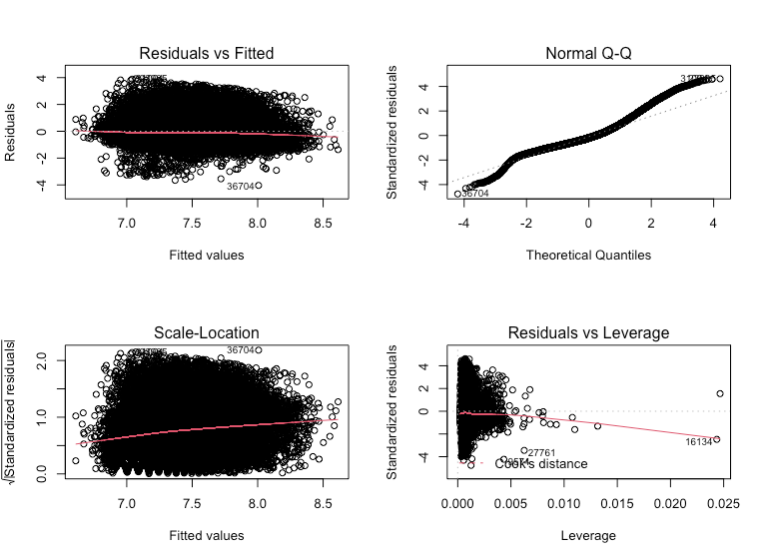
\includegraphics[width=6cm]{7.png} }}%
    \qquad
    \subfloat[Without outliers]{{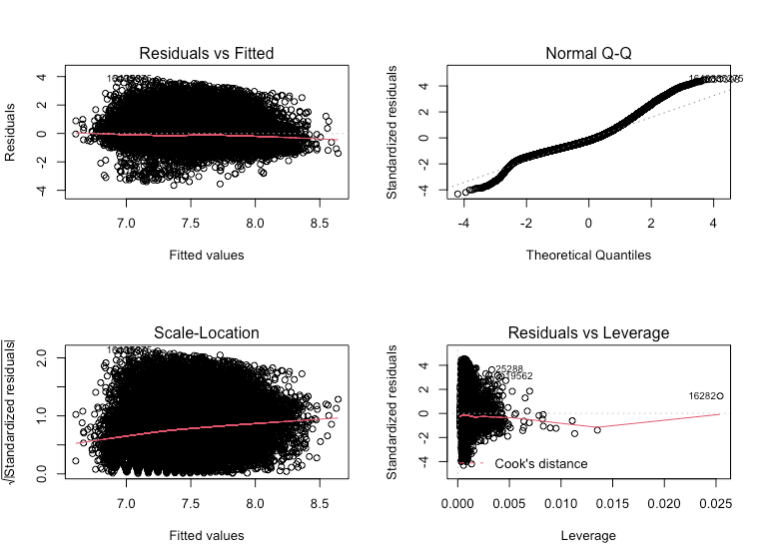
\includegraphics[width=6cm]{7.2.png} }}%
    \caption{Summary Plots of linear regression model}%
    \label{fig7}%
\end{figure}
The summary plots of the model: fig.\ref{fig7} show that the data set has some outliers or high leverage points that may affect the fitted line. After deleting these points, the model still does not seem to fit well. The QQ plot shows that the residual does not follow normal distribution well and the Scale-Location curve is not horizontal. The final model gives a R-square value around 10 percent, which is very low. The predict result using the test set also performs bad, with a MSE of 0.722 (When the share data has taken log). The unfortunate result shows that linear model is not capable of interpreting the high variance of the data.

To improve the linear model, the relationship between variables are also taken into account. Since there. are too many subsets, we then applied forward selection to choose a relatively good model. The selection criterion is still BIC. In the end, there are 40 predictors selected. The summary plots of the model is shown in fig.\ref{fig8}:
\begin{figure}
\centering
    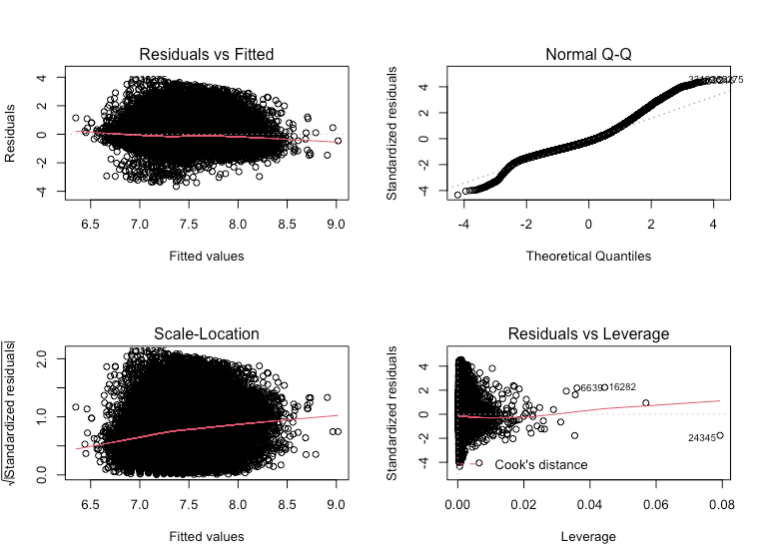
\includegraphics[width=0.7\linewidth]{8.png}
    \caption{Summary Plots of model with interaction terms}
    \label{fig8}
\end{figure}

There is also the residual plots of linear regression models with/without interaction terms on the test data set in fig.\ref{fig9}
\begin{figure}%
    \centering
    \subfloat[Without interaction terms]{{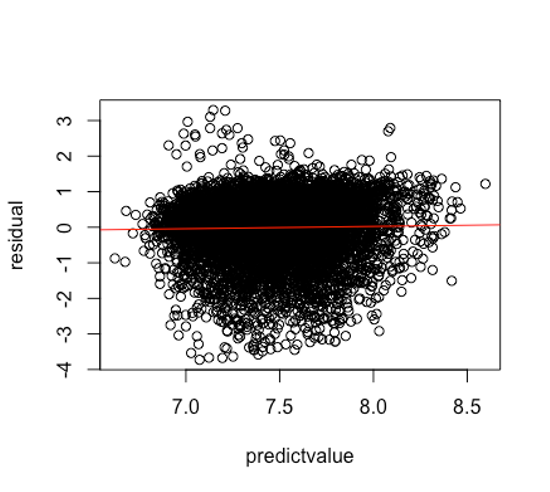
\includegraphics[width=5cm]{9.1.png} }}%
    \qquad
    \subfloat[With interaction terms]{{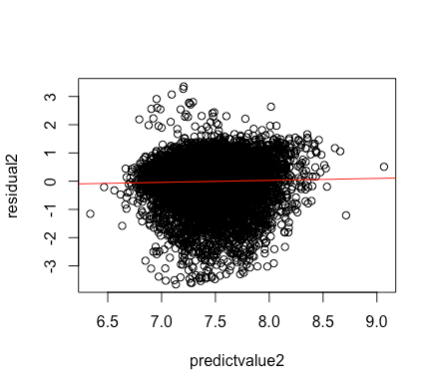
\includegraphics[width=5cm]{9.png} }}%
    \caption{Feature Selection Process of Linear Regression}%
    \label{fig9}%
\end{figure}

These plots show that the model shares the same question with the previous model, which further indicates that linear model is not suitable for the data. The R-square is a little bit higher than the previous model, but still around 10 percent. The MSE on the test data is 0.716, improved a little bit. Thus, we further move on to some non-linear models.

\subsection{Generalized Linear Regression}
In this section, we considered classification model to try for improvement in accuracy. In the first part, 3 models of logistic regression are applied, where response “share” is classified in 2, 3 and 4 groups. In the second part, the possibility of other families in GLM were examined. 
\subsubsection{Logistic Regression}
First we conducted data categorization. The threshold of the classification is obtained from the median of data sample in terms of the 2-category case. And for the 3-category case, the thresholds are 33.33\% quantile and 66.67\% quantile, while the one in 25\%, 50\% and 75\% quantile for the 4-category case. Details are shown in the following table:
\begin{center}
 \begin{tabular}{||c c c ||} 
 \hline
 Cases & Response(y) & Threshold \\ [0.5ex] 
 \hline\hline
 2 categories (Binomial) & 0,1 & \makecell[c]{$0 = y\leq$ median\\ $1 = y >$ median} \\ 
 \hline
 3 categories & 1,2,3 & \makecell[c]{$1 = y \leq 33.33\%$ quantile\\
$2 = 33.33\% $quantile $< y \leq 66.67\%$ quantile\\
$3 = y > 66.67\%$ quantile} \\
 \hline
 4 categories & 1,2,3,4 & \makecell[c]{$1 = y \leq 25\%$ quantile\\
$2 = 25\%$ quantile $< y \leq 50\%$ quantile\\
$3 = 50\%$ quantile $< y \leq 75\%$ quantile\\
$4 = y > 75\%$ quantile }\\ [1ex] 
 \hline
\end{tabular}
\end{center}

Next is feature Selection step. In order to handle the multicollinearity problem and make variable selection simultaneously, the elastic net method is carried out based on the modified data in the logistic regression part. Instead of using the original least square solution method, the elastic net method adds the penalty to the formula, where the target of the solution becomes:
\[
\sum_{t=1}^{n}\left(y_{t}-\beta_{0}-\beta_{1} x_{1 t}-\ldots-\beta_{p} x_{p t}\right)^{2}+\lambda\left[\text { а }|\beta|+(1-\alpha) \beta^{2}\right]
\]
It combines the strengths of lasso and ridge regression and can help to obtain a suitable variable subset for the logistic regression.

In the binomial step, the model with elastic net method pick 37 out of 59 variables. Noticeably, the predictors “n\_unique\_tokens” and “LDA\_01 ” show insignificant with the response, where their p-values are 0.85 and 0.57 respectively. One of the attempt to deal with it is to directly delete them and construct a new logistic regression model with the remaining predictors. However, the anova test of these two model shows that the improvement of the latter model is not as expected (p-value=0.84). In addition, the performance marginal model plots shown in fig.\ref{fig10} and the ROC curve are acceptable. Hence, the logistic model with 37 predictors is finally picked.
\begin{figure}
\centering
    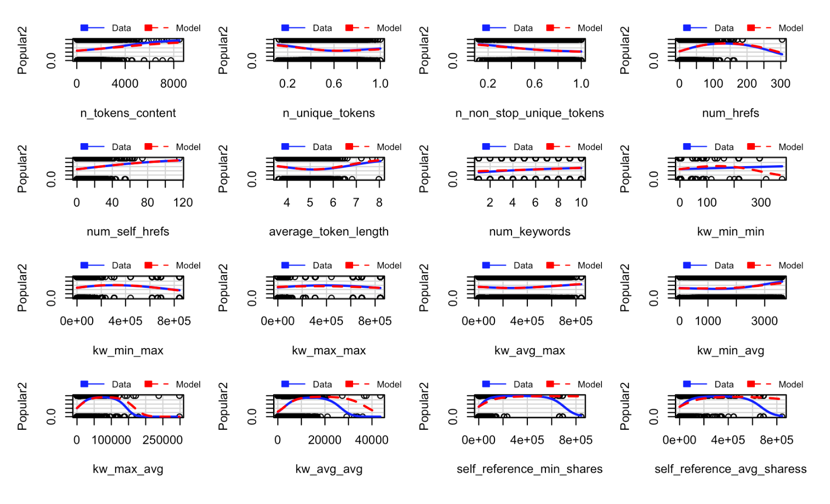
\includegraphics[width=0.7\linewidth]{10.1.png}
    %\caption{Summary Plots of model with interaction terms}
    %\label{fig10}
\end{figure}
\begin{figure}
\centering
    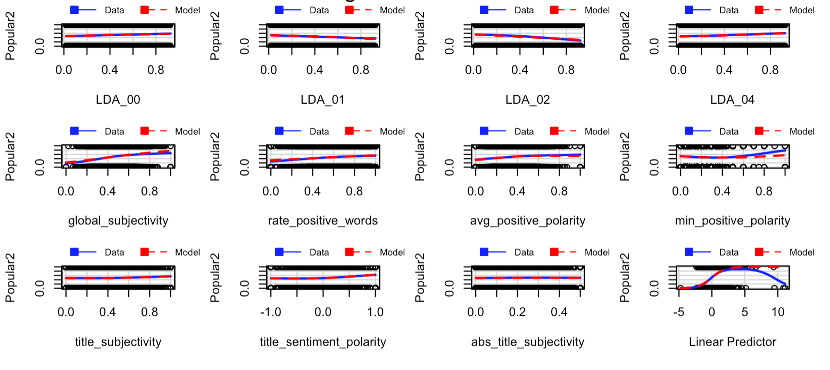
\includegraphics[width=0.7\linewidth]{10.2.png}
    \caption{Marginal Model Plots}
    \label{fig10}
\end{figure}

With the threshold of 0.467 calculated with AUC displayed in fig.\ref{fig11}, the misclassification rate of the logistic model is around 0.35.
\begin{figure}
\centering
    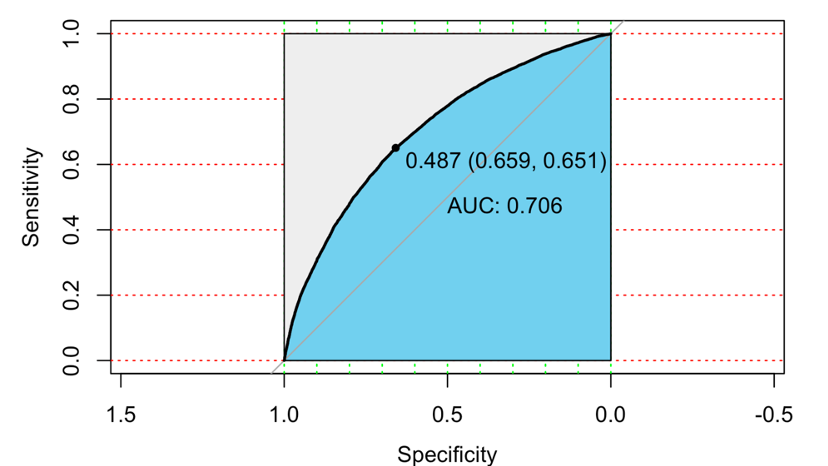
\includegraphics[width=0.7\linewidth]{11.png}
    \caption{ROC Curve of Logistic Regression Model}
    \label{fig11}
\end{figure}

For multinomial classifications (say k classes), the model uses logarithmic function to estimate the relative probability of each category with reference to the kth category. We applied similar process in the multinomial logistic regression of 3 categories and 4 categories. Their misclassification rate is around 0.51 and 0.62 as shown in the table below. Since the misclassification rate shows a growing trend as the number of category increases, from the business perspective, the accuracy also plays a key role in prediction of the popular post which would result in more views and more business. Thus, considering accuracy as a primary factor, the models built with 2 categories are chosen.
\[\begin{tabular}{|l||l||l||l|}
\hline & Logistic & Multinomial & Multinomial \\
& & & \\
& \((2\) categories) & \((3\) categories) & \((4\) categories) \\
\hline & & & \\
& & & \\
Misclassification rate & 0.3455 & 0.5086 & 0.6184  \\
& & & \\
\hline
\end{tabular}\]

\subsubsection{Other Families in GLM}
In addition to 'binomial' family in GLM, we also considered other family options (gamma, Poisson, and Inverse Gaussian) in GLM in this section. First, since the mean of variance of target variable differ a lot, thus it does not satisfy Poisson distribution, thus we rule out this possibility. 

Next we test whether target data satisfy gamma distribution. After generating the qq plot\ref{fig3} comparing log normal and gamma, a conclusion can be drawn that gamma family of GLM is not better than linear regression with log transformation. 
\begin{figure}
\centering
    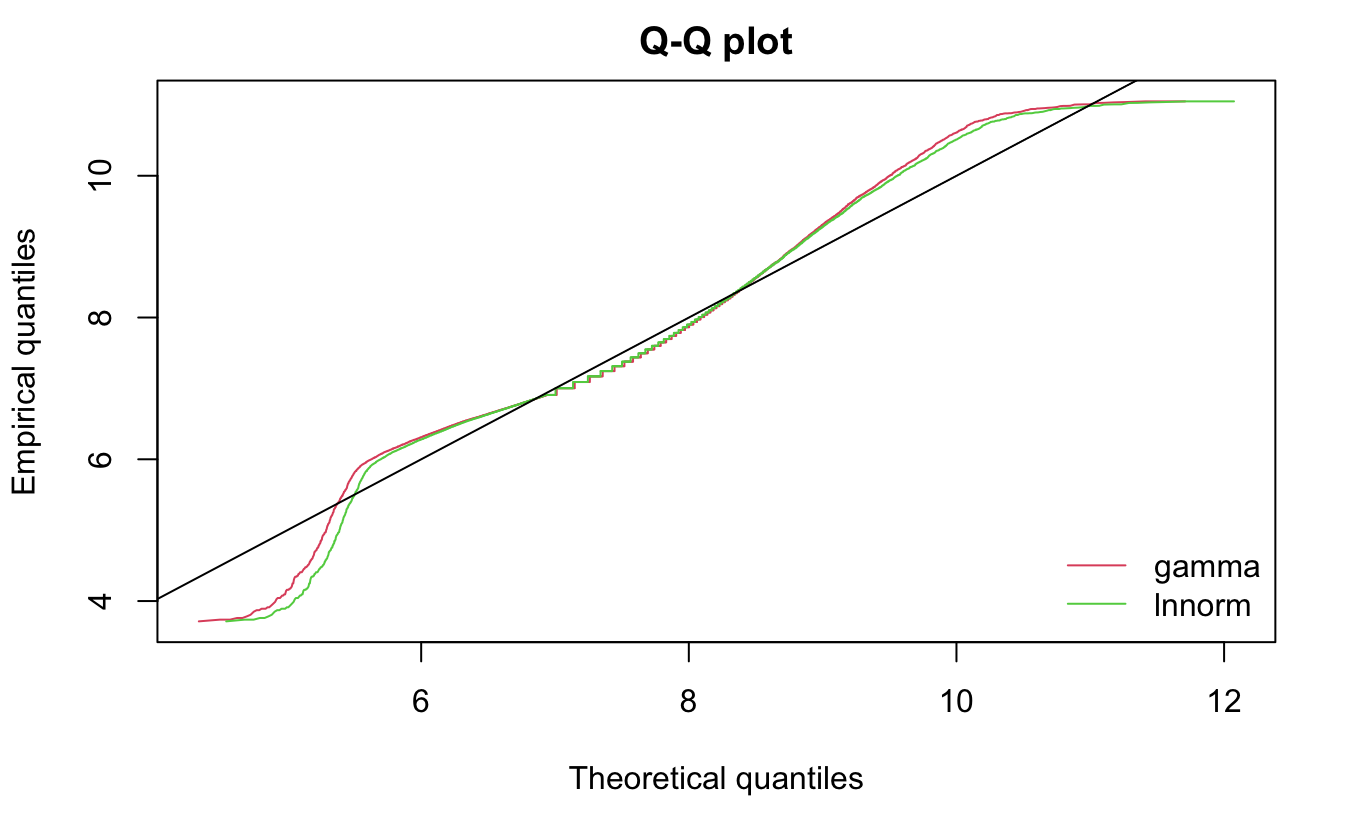
\includegraphics[width=0.7\linewidth]{3.png}
    \caption{qq plot of GLM-Poisson and Log-Normal}
    \label{fig3}
\end{figure}

Finally, we test whether target data fit the 'Inverse Gaussian' family. By conducting the goodness of fit test, we got p-value $<$ 2.2e-16, which rejected the hypothesis. Through this process, we ruled out the possibility of other families in generalized linear model, figured out binomial family is our final choice. 

\subsection{Kernel Method}
In this section, considering the significant difference between features, we fitted a kernel model to the data.
\subsubsection{Feature Selection}
In this section, we selected features through filter method. We used fisher score as our criteria to select features. Fish score for jth feature is given by \cite{a3}:
\[
F(j)=\frac{\left(\bar{x}_{j}^{1}-\bar{x}_{j}^{2}\right)^{2}}{\left(s_{j}^{1}\right)^{2}+\left(s_{j}^{2}\right)^{2}}
\] where
\[
\left(s_{j}^{k}\right)^{2}=\sum_{x \in X^{k}}\left(x_{j}-\bar{x}_{j}^{k}\right)^{2}
\]
The numerator indicates the discrimination be- tween popular and unpopular news, and the de- nominator indicates the scatter within each class. The larger the F-score is, the more likely this feature is more discriminative. We selected the top 20 features with highest score as our features in kernel method. The plot of selected features are in fig.\ref{fig5}
\begin{figure}
\centering
    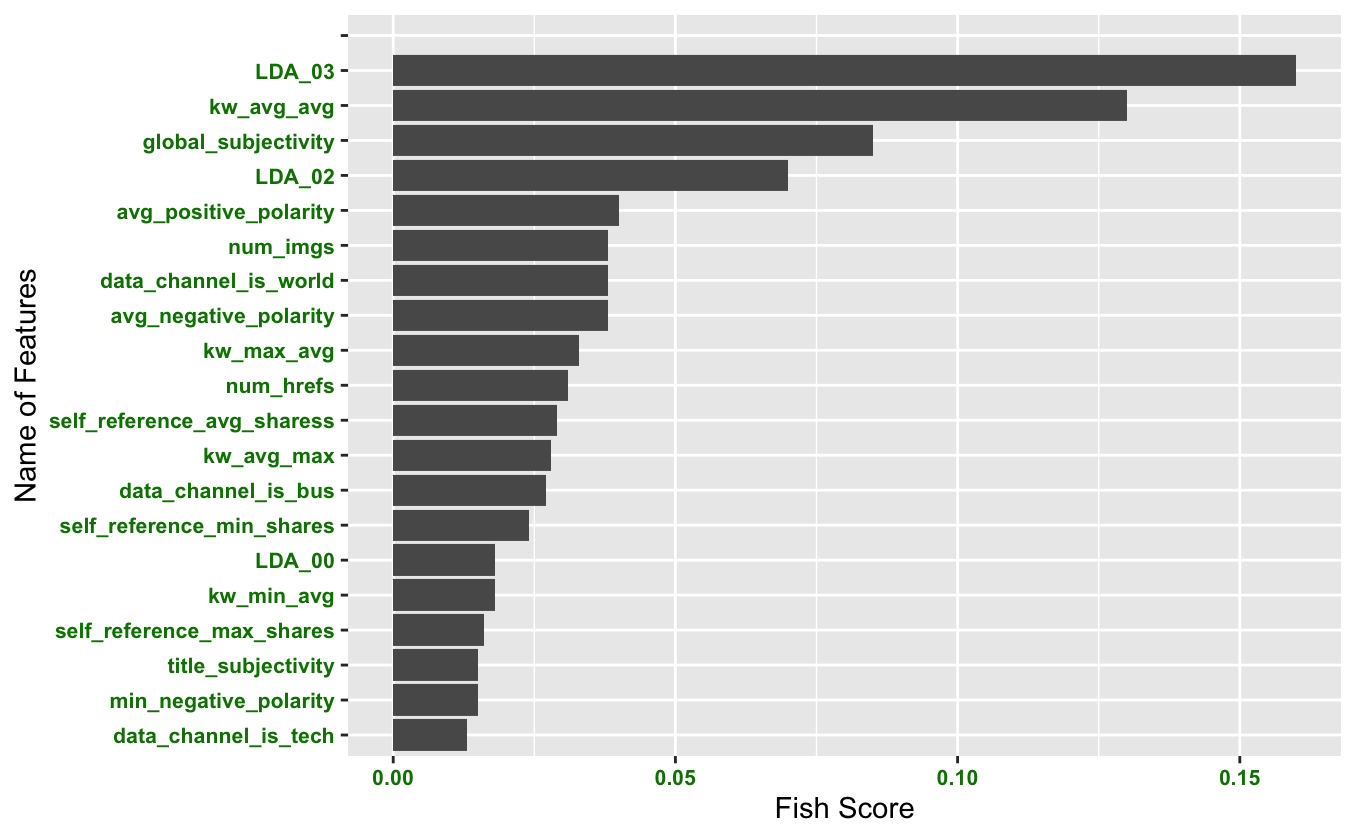
\includegraphics[width=0.7\linewidth]{5.png}
    \caption{Top 20 features selected with Fish Score}
    \label{fig5}
\end{figure}

\subsubsection{Results Analysis}
We choose natural spline as the transformation method for its convenience.  For the natural spline function, the main parameter to be considered is the degree of freedom. The more dispersive a predictor is, the larger degree of freedom is needed for its transformation. Since the features we took are the first 20 features selected through fisher score. Thus, there is different priority level among all features. The method we selected the degree of freedom is exhaustive, that is, we applied all the index from the first feature to the last one. The range of the index for natural spline is from null to 5. The criteria we used for evaluation of results is the MSE on test set (test-MSE). The final model we selected provide a test-MSE of 0.6954774. The plot of residual versus fitted value shows quite uniform distribution around 0 and there is no bad leverage point \ref{fig4}. One thing needs to pay attention is the gradually increasing variance of the residuals.  
\begin{figure}
\centering
    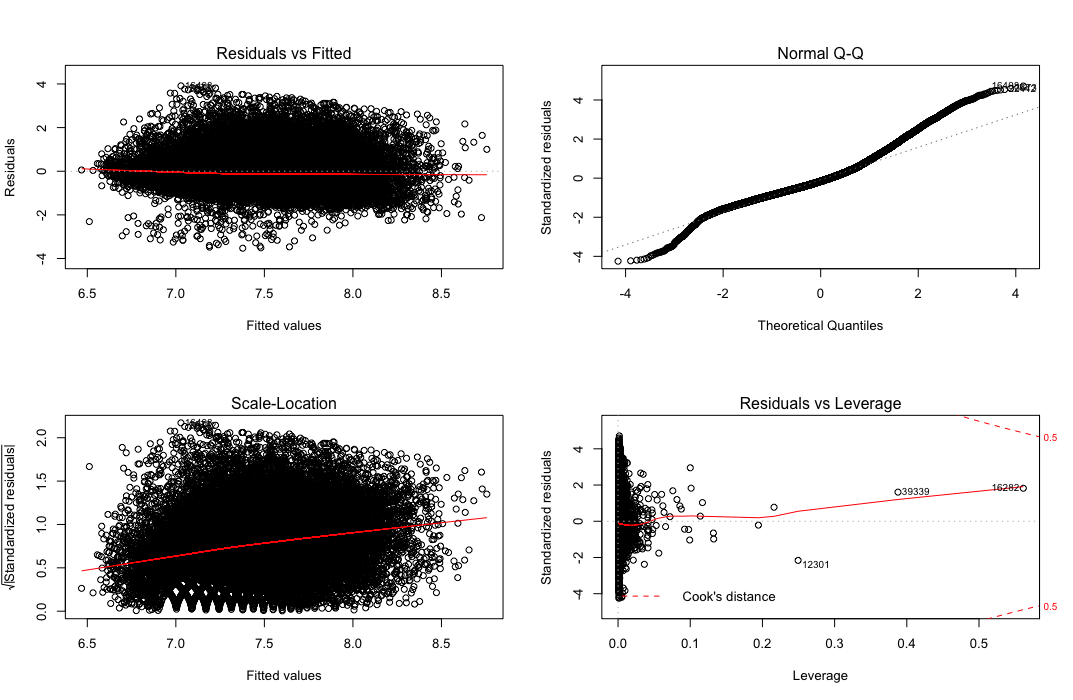
\includegraphics[width=0.7\linewidth]{4.png}
    \caption{Summary Plots from Kernel Method}
    \label{fig4}
\end{figure}

\section{Results}
In this project, we implemented three methods to predict the popularity of online news. Linear regression model and kernel method predict the values of shares, and logistic regression model is regarded as classification method which determines the level of popularity of news articles. 

As a classification model, logistic regression achieves a decent accuracy, better than most of the models. Its Receiver Operating Characteristic Curve is shown in Fig. 3. The AUC value is 0.706, which means logistic regression gives fairly good result when applied in two-category case. Thus, logistic regression model can be selected as a decent classification model.  

By observing training and test error, we can see that the final model linear regression has a MSE value of 0.716 on test set and Kernel method has a MSE value of 0.695 on test set. Due to the large variance of dataset and multicolinearity between attributes, kernel method slightly outperforms linear regression method on the prediction task. 

\section{Future Work}
As it can be seen from the final results of three methods, the highest accuracy we can reach is still low (less than 70\%) based on the data set. Thus, there is still much room for improvement. First, the process of feature selection can still be improved with more advanced methods, perhaps PCA can be applied first to reduce the dimension of parameters; Based on the models we have, we can see that the true content of the articles are not fully explored yet. Variables like LDA only reflect a small portion of articles information. Thus, additional features might be added. In the aspect of model construction, we may consider further apply some machine learning methods like Random Forest, Naive Bayes, some of which have proved better results in other research \cite{a2}. 


%++++++++++++++++++++++++++++++++++++++++
% References section will be created automatically 
% with inclusion of "thebibliography" environment
% as it shown below. See text starting with line
% \begin{thebibliography}{99}
% Note: with this approach it is YOUR responsibility to put them in order
% of appearance.

\begin{thebibliography}{99}

\bibitem{a1}
Tatar, Alexandru, et al. \textit{Predicting the popularity of online articles based on user comments.},International Conference on Web Intelligence, Mining and Semantics. ACM, 2011.

\bibitem{a2}
James, Gareth, et al. \textit{An introduction to statistical learning.},2015 Stanford CS229 project.

\bibitem{a3}
He Ren, Quan Yang \textit{Predicting and Evaluating the Popularity of Online News},New York: springer, 2013.

\end{thebibliography}

\newpage
\appendix
\section{Code for Data Preprocessing}
\definecolor{dkgreen}{rgb}{0,0.6,0}
\definecolor{gray}{rgb}{0.5,0.5,0.5}
\definecolor{mauve}{rgb}{0.58,0,0.82}

\lstset{frame=tb,
  language=R,
  aboveskip=3mm,
  belowskip=3mm,
  breaklines=true,
  showstringspaces=false,
  columns=flexible,
  basicstyle={\small\ttfamily},
  numbers=none,
  numberstyle=\tiny\color{gray},
  keywordstyle=\color{blue},
  commentstyle=\color{dkgreen},
  stringstyle=\color{mauve},
  breakautoindent=true,
  breakatwhitespace=false,
  tabsize=3,
}

\begin{lstlisting}
onlineNews <- read.csv("OnlineNewsPopularity.csv",header = TRUE)
onlineNews<-onlineNews[onlineNews[,4]!=0,]
onlineNews <- onlineNews[,-1]
# remove outliers
onlineNews<-onlineNews[onlineNews[,6]<=1,]

#normalze the target variable 
onlineNews$transformed_shares<-log(onlineNews$shares)

attach(onlineNews)
par(mfrow=c(1,2))
boxplot(onlineNews$shares,names = "Shares",main="Box plot on number of shares",
        ylab="number of shares",sub="Before transformation")
boxplot(transformed_shares,names = "Shares",main="Box plot on number of shares",
        ylab="number of shares",sub="After transformation")
# Remove outliers in targets
boxplotstats<-boxplot(onlineNews$transformed_shares)$stats
print(boxplotstats)
minimum<-boxplotstats[,1][1]
lowerhinge<-boxplotstats[,1][2]
median<-boxplotstats[,1][3]
upperhinge<-boxplotstats[,1][4]
maximum<-boxplotstats[,1][5]

# identify fences
IQR<-upperhinge-lowerhinge
lowerouterfence<-lowerhinge-3*IQR
upperouterfence<-upperhinge+3*IQR
print(IQR)
print(lowerouterfence)
print(upperouterfence)

# remove values beyond fences
onlineNews<-onlineNews[!(onlineNews$transformed_shares>=upperouterfence | onlineNews$transformed_shares<=lowerouterfence),]
boxplot(onlineNews$transformed_shares,xlab="Transformed Shares",main="Shares after ouliers removal")
\end{lstlisting}

\section{Code for Linear Regression}

\begin{lstlisting}
for(i in c(4,9,10,11,21,23,24,27,28,29,30,31,52))
{
  if(min(modifiedData[i])==0){
    print(names(modifiedData[i]))
    modifiedData[i]<-sqrt(modifiedData[i]); names(modifiedData)[i] <- paste("sqrt_",names(modifiedData)[i], sep="")
  }
  else{
    print(names(modifiedData[i]))
    modifiedData[i]<-log(modifiedData[i]); names(modifiedData)[i] <- paste("log_",names(modifiedData)[i], sep="")
  } 
}

#Transformation
modifiedData[8]<-log(modifiedData[8]+1)
names(modifiedData)[8]<- paste("sqrt_",names(modifiedData)[8], sep="")

validattrs<-3:62
validset<-modifiedData[validattrs]

fit1<-lm(normalizedshares~.,data=validset)
summary(fit1)

colinear <- c(4,36,37,42)
validset2<-validset[-colinear]
fit1<-lm(normalizedshares~.,data=validset2)
summary(fit1)
vif(fit1)

plot(sort(vif(fit1)), ylab = 'vif of fit', type='h')
abline(h=5,col='red')


#delete some highly dependent attributes
fit2<-lm(normalizedshares~n_tokens_title+sqrt_num_hrefs+sqrt_num_self_hrefs+sqrt_num_imgs+sqrt_num_videos+average_token_length+num_keywords+data_channel_is_lifestyle+data_channel_is_entertainment+data_channel_is_socmed+kw_min_min+sqrt_kw_max_min+kw_avg_min+sqrt_kw_min_max+sqrt_kw_max_max+kw_avg_max+kw_min_avg+weekday_is_monday+weekday_is_tuesday+weekday_is_wednesday+weekday_is_thursday+weekday_is_friday+weekday_is_saturday+LDA_00+LDA_01+LDA_02+LDA_04+global_subjectivity+global_rate_positive_words+avg_positive_polarity+sqrt_min_positive_polarity+max_positive_polarity+min_negative_polarity+max_negative_polarity+title_subjectivity+title_sentiment_polarity+abs_title_subjectivity+abs_title_sentiment_polarity)

vif(fit2)
plot(sort(vif(fit2)), ylab = 'vif of fit', type='h')

regfit.full<-regsubsets(normalizedshares~n_tokens_title+sqrt_num_hrefs+sqrt_num_self_hrefs+sqrt_num_imgs+sqrt_num_videos+average_token_length+num_keywords+data_channel_is_lifestyle+data_channel_is_entertainment+data_channel_is_socmed+kw_min_min+sqrt_kw_max_min+kw_avg_min+sqrt_kw_min_max+sqrt_kw_max_max+kw_avg_max+kw_min_avg+weekday_is_monday+weekday_is_tuesday+weekday_is_wednesday+weekday_is_thursday+weekday_is_friday+weekday_is_saturday+LDA_00+LDA_01+LDA_02+LDA_04+global_subjectivity+global_rate_positive_words+avg_positive_polarity+sqrt_min_positive_polarity+max_positive_polarity+min_negative_polarity+ max_negative_polarity+title_subjectivity+title_sentiment_polarity+abs_title_subjectivity+abs_title_sentiment_polarity, data=validset,nvmax = 30)

regsum<- summary(regfit.full)
# to simplify model, apply BIC
regsum$bic

print(regsum$which[26,])

reduced<-lm(normalizedshares~sqrt_num_hrefs+sqrt_num_self_hrefs+sqrt_num_imgs+sqrt_num_videos+average_token_length+num_keywords+data_channel_is_entertainment+data_channel_is_socmed+kw_min_min+sqrt_kw_max_min+sqrt_kw_min_max+sqrt_kw_max_max+kw_avg_max+kw_min_avg+sqrt_kw_max_max+kw_avg_max+kw_min_avg+weekday_is_monday+weekday_is_tuesday+weekday_is_wednesday+weekday_is_thursday + weekday_is_friday+LDA_00+LDA_02+global_subjectivity+sqrt_min_positive_polarity+title_subjectivity+title_sentiment_polarity+abs_title_subjectivity)

sum1<- summary(reduced)
par(mfrow=c(2,2))
plot(reduced)

#remove high leverage points, 36704, 23985, 31004, 16134, 27761, 9574
validset<-validset[-c(9574,16134,31004,23985,36704,27761,16120),]
fit3<-lm(normalizedshares~sqrt_num_hrefs+sqrt_num_self_hrefs+sqrt_num_imgs+sqrt_num_videos+average_token_length+num_keywords+data_channel_is_entertainment+data_channel_is_socmed+kw_min_min+sqrt_kw_max_min+sqrt_kw_min_max+sqrt_kw_max_max+kw_avg_max+kw_min_avg+sqrt_kw_max_max+kw_avg_max+kw_min_avg+weekday_is_monday+weekday_is_tuesday+weekday_is_wednesday+weekday_is_thursday + weekday_is_friday+LDA_00+LDA_02+global_subjectivity+sqrt_min_positive_polarity+title_subjectivity+title_sentiment_polarity+abs_title_subjectivity,data=validset)
summary(fit3)
par(mfrow=c(2,2))
plot(fit3)

#predict using test set
set.seed(1)
test=sample(seq(1,length(validset$normalizedshares)), size=0.2*length(validset$normalizedshares),replace = FALSE)
trainset<- validset[-test,]
testset<- validset[test,]
predictlm<-lm(normalizedshares~sqrt_num_hrefs+sqrt_num_self_hrefs+sqrt_num_imgs+sqrt_num_videos+average_token_length+num_keywords+data_channel_is_entertainment+data_channel_is_socmed+kw_min_min+sqrt_kw_max_min+sqrt_kw_min_max+sqrt_kw_max_max+kw_avg_max+kw_min_avg+sqrt_kw_max_max+kw_avg_max+kw_min_avg+weekday_is_monday+weekday_is_tuesday+weekday_is_wednesday+weekday_is_thursday + weekday_is_friday+LDA_00+LDA_02+global_subjectivity+sqrt_min_positive_polarity+title_subjectivity+title_sentiment_polarity+abs_title_subjectivity,data=trainset)
predictvalue<-predict(predictlm,newdata = testset)
mse<-mean((predictvalue-log(testset$shares))^2)

residual<-predictvalue-testset$normalizedshares
plot(predictvalue,residual)
abline(lm(residual~predictvalue),col='red')


#covariate part
covariateset<-validset[c(6,7,8,9,10,11,13,15,18,19,21,22,23,24,30,31,32,33,34,38,40,43,50,55,57,60)]
detach(validset)
attach(covariateset)
fit4<-lm(normalizedshares~.+.^2,data=covariateset)

null<-lm(normalizedshares~1,data=covariateset)

#use BIC to do step functions
fwd<-step(null,scope = formula(fit4),direction = 'forward',k=log(length(fit4$residuals)))
summary(fwd)
par(mfrow=c(2,2))
plot(fwd)

#test sets
testcov<-covariateset[test,]
traincov<-covariateset[-test,]

predictlm2<-lm(formula = formula(fwd), data=traincov)
predictvalue2<-predict(predictlm2,newdata = testcov)
residual2<-predictvalue2-testcov$normalizedshares
plot(predictvalue2,residual2)
abline(lm(residual2~predictvalue2),col='red')
mse=mean(residual2^2)
\end{lstlisting}

\section{Code for Generalized Linear Regression}
\begin{lstlisting}
# Logistic Regression
for (i in c(12:17, 30:37)){
  modified.d[,i] <- as.factor(modified.d[,i])
}

#Use elastic net to find the model (deal with the variable reduction and multicollinearity problem)
library(glmnet)
set.seed(1234)
X_2groups <- data.matrix(modified.d[,-59])
cvfit <- cv.glmnet(X_2groups, modified.d$Popular2, family="binomial")
beta.logistic <- coef(cvfit, s="lambda.1se")
model.logistic <- which(beta.logistic[2:length(beta.logistic)]!=0)
coef <- predict(cvfit, type="coefficients", s="lambda.1se")
sel <- which(coef[,1]!=0)
coef[sel,]
length(sel)

logiSel <- glm(Popular2 ~ n_tokens_content + n_unique_tokens + n_non_stop_unique_tokens + num_hrefs + num_self_hrefs + average_token_length + num_keywords + data_channel_is_entertainment + data_channel_is_bus + data_channel_is_socmed + data_channel_is_tech + kw_min_min + kw_min_max + kw_max_max + kw_avg_max + kw_min_avg + kw_max_avg + kw_avg_avg + self_reference_min_shares + self_reference_avg_sharess + weekday_is_monday + weekday_is_tuesday + weekday_is_wednesday + weekday_is_friday + weekday_is_saturday + is_weekend + LDA_00 + LDA_01 + LDA_02 + LDA_04 + global_subjectivity + rate_positive_words + avg_positive_polarity + min_positive_polarity + title_subjectivity + title_sentiment_polarity + abs_title_subjectivity, data = modified.d, family = "binomial")
summary(logiSel)

#delete the insignificant variables
logiSel0 <- glm(Popular2 ~ n_tokens_content + n_non_stop_unique_tokens + num_hrefs + num_self_hrefs + average_token_length + num_keywords + data_channel_is_entertainment + data_channel_is_bus + data_channel_is_socmed + data_channel_is_tech + kw_min_min + kw_min_max + kw_max_max + kw_avg_max + kw_min_avg + kw_max_avg + kw_avg_avg + self_reference_min_shares + self_reference_avg_sharess + weekday_is_monday + weekday_is_tuesday + weekday_is_wednesday + weekday_is_friday + weekday_is_saturday + is_weekend + LDA_00 + LDA_02 + LDA_04 + global_subjectivity + rate_positive_words + avg_positive_polarity + min_positive_polarity + title_subjectivity + title_sentiment_polarity + abs_title_subjectivity, data = modified.d, family = "binomial")
summary(logiSel0)

#anova test
anova(logiSel0,logiSel)
qchisq(0.95, 2)
1-pchisq(0.33685,2)

par(mfrow=c(2,2))
plot(logiSel)
par(mfrow=c(1,1))
plot(logiSel$fitted.values, rstandard(logiSel))

mmps(logiSel, layout=c(4,4))

#ROC curve and AUC
library(pROC)
pre.logi <- predict(logiSel, type="response")
modelroc <- roc(modified.d$Popular2, pre.logistic)
coords(modelroc, x=0.5)
par(mfrow=c(1,1))
plot(modelroc, print.auc=TRUE, auc.polygon=TRUE, grid=c(0.1, 0.2),
     grid.col=c("green", "red"), max.auc.polygon=TRUE,  
     auc.polygon.col="skyblue", print.thres=TRUE)   #p=0.487

predicted <- rep(0,nrow(modified.d))
predicted[which(pre.logi>=0.487)] <- 1
mis.logi <- table(predicted, modified.d$Popular2)
1-sum(diag(mis.logi))/sum(mis.logi)  #misclassification rate


#multinomial
#3 categories
quantile(modifiedData$shares, probs = c(0.3333,0.6667))
modified.d2 <- modifiedData
modified.d2$Popular3[which(modified.d2$shares>1100 & modified.d2$shares<=2100)] <- 2
modified.d2$Popular3[which(modified.d2$shares<=1100)] <- 1
modified.d2$Popular3[which(modified.d2$shares>2100)] <- 3
modified.d2$Popular3 <- as.factor(modified.d2$Popular3)
modified.d2 <- modified.d2[,-59]

library(glmnet)
set.seed(1234)
X_3groups <- data.matrix(modified.d2[,-59])
cvfit.multi <- cv.glmnet(X_3groups, modified.d2$Popular3, family="multinomial")
#beta.multi <- coef(cvfit.multi, s="lambda.1se")
#model.multi <- which(beta.multi[2:length(beta.multi)]!=0)
multi.model <- glmnet(X_3groups, modified.d2$Popular3, family="multinomial", lambda = cvfit.multi$lambda.1se)
pre.multi <- predict(cvfit.multi, X_3groups, s="lambda.1se", type="class")
mis.multi <- table(pre.multi, modified.d2$Popular3)
mis.multi
1-sum(diag(mis.multi))/sum(mis.multi)  #misclassification rate


#4 categories
quantile(modifiedData$shares, probs = c(0.25, 0.5, 0.75))
modified.d3 <- modifiedData
modified.d3$Popular4[which(modified.d3$shares>944 & modified.d3$shares<=1400)] <- 2
modified.d3$Popular4[which(modified.d3$shares <= 944)] <- 1
modified.d3$Popular4[which(modified.d3$shares>1400 & modified.d3$shares<=2700)] <- 3
modified.d3$Popular4[which(modified.d3$shares>2700)] <- 4
modified.d3$Popular4 <- as.factor(modified.d3$Popular4)
modified.d3 <- modified.d3[,-59]

library(glmnet)
set.seed(1234)
X_4groups <- data.matrix(modified.d3[,-59])
cvfit.multi4 <- cv.glmnet(X_4groups, modified.d3$Popular4, family="multinomial")
#beta.multi <- coef(cvfit.multi, s="lambda.1se")
#model.multi <- which(beta.multi[2:length(beta.multi)]!=0)
multi4.model <- glmnet(X_4groups, modified.d3$Popular4, family="multinomial", lambda = cvfit.multi4$lambda.1se)
pre.multi4 <- predict(cvfit.multi4, X_4groups, s="lambda.1se", type="class")
mis.multi4 <- table(pre.multi4, modified.d3$Popular4)
mis.multi4
1-sum(diag(mis.multi4))/sum(mis.multi4)  #misclassification rate

# Testing of other families in GLM
# test normality
library("ggpubr")
ggdensity(onlineNews$transformed_shares, 
          main = "Density plot of transformed shares",
          xlab = "log number of shares")
ggqqplot(onlineNews$transformed_shares)

ggdensity(onlineNews$shares, 
          main = "Density plot of shares",
          xlab = "number of shares")
ggqqplot(onlineNews$shares)

# Test Gamma
library(fitdistrplus)
descdist(onlineNews$transformed_shares, boot=1000)

# further test
gammafit  <-  fitdistrplus::fitdist(onlineNews$transformed_shares, "gamma")
lnormfit  <-  fitdistrplus::fitdist(onlineNews$transformed_shares, "lnorm")  

library(flexsurv) 

qqcomp(list(gammafit, lnormfit),
       legendtext=c("gamma","lnnorm") )
       
# Test Inverse Gaussian
library(goft)
ig_test(sample(onlineNews$transformed_shares,5000), method = "transf")
\end{lstlisting}

\section{Code for Kernel Method}
\begin{lstlisting}
# Calculation of Fish Score
library(PredPsych)
library(ggplot2)
onlineNews$class <- NA
for (i in 1:nrow(onlineNews)) {
  if (onlineNews$shares[i] <= 14000){
      onlineNews$class[i] = 0
    }else{onlineNews$class[i] = 1}
}
fscore <- fscore(onlineNews, classCol = 62, featureCol = c(1:59))
fscore20 <-read.csv("fs.csv",header = TRUE)
attach(fscore20)
y <-fscore20$fscore
ggplot(fscore20, aes(x = features, y = fscore, main="Feature Scores")) +
         geom_bar(aes(reorder(features,fscore),fscore),stat = "identity") +
         coord_flip() + scale_y_continuous(name="Fish Score") +
  scale_x_discrete(name="Name of Features") +
theme(axis.text.x = element_text(face="bold", color="#008000",
                           size=8, angle=0),
          axis.text.y = element_text(face="bold", color="#008000",
                           size=8, angle=0))
# Kernel Method Application
library(gam)
library(splines)

set.seed(1)
train<-sample(nrow(modifiedData),0.8*nrow(modifiedData),replace=FALSE)
train_data<-modifiedData[train,]
test_data<-modifiedData[-train,]

fisher.gam1 <- lm(log(shares)~ns(kw_avg_avg,3)+ns(LDA_02,3)+data_channel_is_world+is_weekend+data_channel_is_socmed+weekday_is_saturday+ns(LDA_04,3)+ns(data_channel_is_entertainment,3)+data_channel_is_tech+ns(kw_max_avg,4)+weekday_is_sunday+ns(LDA_00,3)+ns(num_hrefs,3)+ns(global_subjectivity,3)+ns(kw_min_avg,3)+ns(global_sentiment_polarity,3)+ns(rate_negative_words,3)+ns(kw_min_min,3)+ns(title_subjectivity,3)+ns(LDA_01,3),data=train_data)

summary(fisher.gam1)

fisher.gam2 <- lm(log(shares)~ns(kw_avg_avg,5)+ns(LDA_02,3)+data_channel_is_world+is_weekend+data_channel_is_socmed+weekday_is_saturday+ns(LDA_04)+ns(data_channel_is_entertainment)+data_channel_is_tech+ns(kw_max_avg,4)+weekday_is_sunday+LDA_00+ns(num_hrefs)+ns(global_subjectivity)+ns(kw_min_avg,3)+ns(global_sentiment_polarity)+rate_negative_words+ns(kw_min_min)+ns(title_subjectivity,2)+LDA_01,data=train_data)

summary(fisher.gam2)

anova(fisher.gam2,fisher.gam1)
options(warn=-1) 
gam.pred <- predict(fisher.gam2,newdata=test_data)
gam.mse=mean((gam.pred-test_data$shares)^2)
\end{lstlisting}
\end{document}
